\chapter{Performance MIDI-to-Score Conversion by Neural Beat Tracking}

The main model of interest \cite{Liu2022}, developed by Liu et al. (2022), is a state-of-the-art machine learning model for complete music transcription. It has been awarded as the best paper of the \emph{International Society for Music Information Retrieval Conference} (ISMIR) in December 2022.

The model is composed of two parts:
\begin{itemize}
	\item Beat Tracking.
	\item Score Element Assignment.
\end{itemize}

The first part is responsible for quantizing the raw material into beats and downbeats. Each measure is consisted of several beats, and the number of beats in a measure is governed by the time signature. The beats mark the tempo, and they are the basis for the musical onsets detection.

The second part assigns every other aspect of the musical score to the MIDI stream. Let us recall these elements: musical onsets, note values, hand parts, key signature and time signature.

Let us review both components.

\section{Beat Tracking}

A single measure consists of several beats, and the rhythmic structure of beats is determined by time signature (or signatures). A performance MIDI does not contain information about beats and one of the objectives of the model is to predict locations of these.

After these predictions, note beginnings (onsets) can be placed in a subdivision of a single beat. The smallest unit of time distance is thus dictated by the size of the beat subdivision. More precisely, a musical onset $mo_i$ of the $i$-th note is defined as \[mo_i = \frac{s_n}{S}\] where $S$ is the number of subdivisions per beat in rhythm quantization, and $s_n$ is the musical onset time expressed in the number of subdivisions.

The authors provide a novel approach to detecting beats, splitting them into two categories, for which there are two separate methods.

Beats can fall into two distinct groups:
\begin{itemize}
	\item \emph{In-note}: beats concurrent with at least one note onset. This means that some notes play within the start of the beat.
	\item \emph{Out-of-note}: a beat is not concurrent with any note onset. No notes are beginning with such beats.
\end{itemize}

\subsection{In-note Beat Prediction}

For predicting in-note beats, one can reduce the problem to a binary classification task on the note sequence $\mathbf{X}$. This sequence is assumed to have a length $N$.

\begin{figure}[!ht]
\centering
\begin{tikzpicture}
\tikzset{layer1/.style={fill=gray!10, draw=gray, thick, text centered}}
\tikzset{layer2/.style={fill=gray!30, draw=gray, thick, text centered}}
\tikzset{arrowstyle/.style={-{Latex[length=3mm]}}}

	\fill[fill=gray!50, fill opacity=0.5, draw=gray, thick, line width=2pt] (0.0, 0.0) rectangle (12.0, 7.0);
	\fill[fill=gray!30, fill opacity=0.5, draw=gray, thick, line width=2pt] (0.0, -0.5) rectangle (12.0, -4.0);
	\fill[fill=white!50, fill opacity=1.0, draw=black, thick, line width=1pt] (0.5, 2.0) rectangle (10.5, 6.5);
	\fill[fill=white!50, fill opacity=1.0, draw=black, thick, line width=1pt] (1.0, 1.5) rectangle (11.0, 6.0);
	\fill[fill=white!50, fill opacity=1.0, draw=black, thick, line width=1pt] (1.5, 1.0) rectangle (11.5, 5.5);

    \draw (6.5, 7.75) node (note_sequence) {Note sequence};
    \draw (6.5, 4.75) node[layer2] (layerA1) {Convolutional};
    \draw (6.5, 3.75) node[layer1] (layerA2) {Batch normalization};
    \draw (6.5, 2.75) node[layer1] (layerA3) {Exponential linear unit};
    \draw (6.5, 1.75) node[layer1] (layerA4) {Dropout};
    \draw[anchor=south, inner sep=2pt] (6.5, 0.0) node (outputA) {To the next convolutional layer};
    
    \draw (6.5, -1.25) node[layer2] (layerB1) {Bi-directional GRU (512)};
    \draw (6.5, -2.25) node[layer2] (layerB2) {Bi-directional GRU (512)};
    \draw (6.5, -3.25) node[layer1] (layerB3) {Linear (512)};
    
    \draw (6.5, -5.00) node[layer1] (output) {Linear (1)};
    
	\node[anchor=south west, inner sep=2pt] at (0.2, 0.2) {ConvBlock};    
	\node[anchor=south west, inner sep=2pt] at (0.2, -3.8) {GRUBlock};
	
	\node[anchor=north west, inner sep=2pt] at (1.55, 5.45) {\small{(9, in features), 128}};
	\node[anchor=north west, inner sep=2pt] at (1.05, 5.95) {\small{(9, 1), 256}};
	\node[anchor=north west, inner sep=2pt] at (0.55, 6.45) {\small{(9, 1), 512}};
	\node[anchor=north west, inner sep=2pt] at (0.05, 6.95) {\small{kernel size, channels}};
	
	\draw[arrowstyle] (note_sequence.south) to (layerA1.north);
	\draw[arrowstyle] (layerA1.south) to (layerA2.north);
	\draw[arrowstyle] (layerA2.south) to (layerA3.north);
	\draw[arrowstyle] (layerA3.south) to (layerA4.north);
	\draw[arrowstyle] (layerA4.south) to (outputA.north);
	\draw[arrowstyle] (layerA4.south) to (outputA.north);
	
	\draw[arrowstyle] (outputA.south) to (layerB1.north);
	\draw[arrowstyle] (layerB1.south) to (layerB2.north);
	\draw[arrowstyle] (layerB2.south) to (layerB3.north);
	\draw[arrowstyle] (layerB3.south) to (output.north);
\end{tikzpicture}
\caption[In-note beat prediction model]{In-note beat prediction model with a CRNN with 3 convolutional layers and 2 bi-directional gated recurrent unit (GRU) layers.}
\end{figure}

The probability $P_n$ that $n$-th note is concurrent with a beat is defined as: \[P_n = \mathbb{P}\left(B_n|\mathbf{X}\right)\] where $B_n\in\{0,1\}$ is the ground-truth beat label for the $n$-th note from the note sequence. The model is trained using the standard cross-entropy loss function: \[\mathcal{L}=-\frac{1}{N}\sum_{n=1}^N B_n\ln P_n + \left(1-B_n\right)\ln\left(1-P_n\right)\] The authors used CRNN with 3 convolutional layers and 2 bidirectional gated recurrent unit (GRU) layers. The probability threshold for positive classification has been set dynamically, depending on the maximum probability in a fixed segment length.

\subsection{Out-of-note Beat Prediction}

The approach to predicting out-of-note beats, which do not align with note onsets, requires distinct approach. Liu et al. (2022) proposed a dynamic programming strategy to solve this problem \cite{Liu2022}.

Let us assume that there are $B^i$ in-note beats $\{b_n^i\}_{n=1}^{B^i}$ in total, and out-of-note beats are at subdivisions of the neighboring in-note beats\footnote{We may select only one note per in-note beat, if there are more.} $b_{n}^i$ and $b_{n+1}^i$.

The goal of the procedure is to find out-of-note beats $b^o$ from a set of candidates: \begin{equation}\label{out_of_note_candidates}
b_{n,K}^o = \left\{b_n^i + \frac{k}{K+1}\left(b_{n+1}^i-b_n^i\right)\right\}_{k=1}^K
\end{equation} where $K\in\{0,1,2,3\}$ is the number of out-of-note beats to insert inside the $\left(b_{n+1}^i, b_n^i\right)$ interval.

The number of candidates is selected in order to minimize the tempo change after adding out-of-note beats. The function may be represented as the sum: \[\mathcal{O}_1 = \sum_{n=1}^{B-2}\left|\ln\left(\frac{b_{n+2} - b_{n+1}}{b_{n+1} - b_n}\right)\right|\] where $\{b_n\}_{n=1}^B$ is the sequence of all $B$ beats (both in-note and out-of-note, sorted chronologically).

To discourage the procedure from adding too many out-of-note beats, which leads to an unnecessarily subdivided output, an additional penalty is associated with the objective function: \begin{equation}\label{out_of_note_objective}
\mathcal{O} = \mathcal{O}_1 + \lambda B^o
\end{equation} where $B^o$ is the number of added out-of-note beats, and $\lambda$ is the penalty coefficient. The coefficient is to be found experimentally, however the default value set by the authors is $1$.

\begin{algorithm}[ht!]
\begin{algorithmic}[1]
\Require{list of in-note notes $\mathcal{B}^i$}
\Ensure{list of all beats $\mathcal{B}$ including added out-of-note beats}
\State $n \gets 1$
\For{$K=0,1,2,3$}
    \State initialize objective function $\mathcal{O}_K\gets 0$
    \State initialize beat sequence $\mathcal{B}_K\gets \{b_1\}$
\EndFor
\For{$n=1,2,\ldots,B^i-2$}
    \For{$K_{\textrm{cur}}=0,1,2,3$}
        \State get out-of-note beats for current step by \eqref{out_of_note_candidates}
        \If{tempo is beyond tempo range limits}
            \State \textbf{continue}
        \EndIf
        \For{$K_{\textrm{prev}}=0,1,2,3$}
            \State update objective function by \eqref{out_of_note_objective}
        \EndFor
        \State select the minimum objective among all $K_{\textrm{prev}}$ values
        \State add out-of-beats for the current step to the beat sequence mapped to the selected $K_{\textrm{prev}}$
    \EndFor
    \For{$K_{\textrm{cur}}=0,1,2,3$}
        \State update $\mathcal{O}_K$, $\mathcal{B}_K$ mapped with $K_{\textrm{cur}}$
    \EndFor
\EndFor
\State \Return{the beat sequence $\mathcal{B}_K$ with the minimum objective function $\mathcal{O}_K$}
\end{algorithmic}
\captionof{algorithm}[Out-of-note beat prediction.]{Out-of-note beat prediction.}
\end{algorithm}


\section{Input Data Encoding}

The entire score needs to be transformed to a suitable data format before passing to any of the model components. Given a note sequence tensor as described earlier, the data is encoded into a variety of features: \begin{itemize}
	\item $128$-dimensional one-hot encoding of MIDI pitches.
	\item One-hot onset time-shift ($o_i - o_{i-1}$) quantised by $10$ ms resolution, with maximum value of $4$ s, $401$ features in total.
	\item Raw duration values in seconds.
	\item Velocities normalized to the unit interval $[0, 1]$.
\end{itemize}

There are $531$ features in total.

The authors tried different encoding schemes, for pitches, onset times and durations, including raw float values in seconds. The full study is available in the paper \cite{Liu2022}.

\section{Score Elements Assignment}

As discussed in the Section \ref{music_score_encoding}, score elements assignment may be viewed as a function from a note sequence $\mathbf{X}$ into a score encoded by a tensor $\mathbf{Y}_n$ representing musical onsets, note values, key signature, time signature, and hand parts, for each note separately.

Besides the quantization model, which relies on the beat tracking module, key signature, time signature and hand parts modules can be treated independently.

\begin{figure}[!ht]
\centering
\begin{tikzpicture}
    \tikzset{sequence/.style={thick, text centered, align=center}}
    \tikzset{convblock/.style={fill=gray!20, draw=gray, thick, text centered}}
    \tikzset{grublock/.style={fill=gray!30, draw=gray, thick, text centered}}
    \tikzset{linear/.style={fill=gray!10, draw=gray, thick, text centered}}
    \tikzset{output/.style={thick, anchor=west, align=left}}
    \tikzset{arrowstyle/.style={-{Latex[length=3mm]}}}
    \draw (-3.5, 0.5) node[sequence] (sequence) {note\\ sequence};

    \draw (-1.75, 5) node (joint1) {};
    \draw (-1.75, 3) node (joint2) {};
    \draw (-1.75, 2) node (joint3) {};
    \draw (-1.75, 0.5) node (joint4) {};
    \draw (-1.75, -1) node (joint5) {};
    \draw (-1.75, -2) node (joint6) {};

    \draw (1.5, 3) node (concatenation) {$\boldsymbol{\oplus}$};
    \draw (1.5, 3.5) node (concatleftjoint1) {};
    \draw (1.5, 2.5) node (concatleftjoint2) {};
    \draw (7.25, 3.5) node (concatrightjoint1) {};
    \draw (7.25, 2.5) node (concatrightjoint2) {};
    \draw (7.25, 2) node (concatstart1) {};
    \draw (7.25, 4) node (concatstart2) {};

    \draw (0, 5) node[convblock] (convblock1) {ConvBlock};
    \draw (0, 3) node[convblock] (convblock2) {ConvBlock};
    \draw (0, 2) node[convblock] (convblock3) {ConvBlock};
    \draw (0, 0.5) node[convblock] (convblock4) {ConvBlock};
    \draw (0, -1) node[convblock] (convblock5) {ConvBlock};
    \draw (0, -2) node[convblock] (convblock6) {ConvBlock};

    \draw (3, 6) node[grublock] (grublock1) {GRUBlock};
    \draw (3, 5) node[grublock] (grublock2) {GRUBlock};
    \draw (3, 4) node[grublock] (grublock3) {GRUBlock};
    \draw (3, 3) node[grublock] (grublock4) {GRUBlock};
    \draw (3, 2) node[grublock] (grublock5) {GRUBlock};
    \draw (3, 0.5) node[grublock] (grublock6) {GRUBlock};
    \draw (3, -1) node[grublock] (grublock7) {GRUBlock};
    \draw (3, -2) node[grublock] (grublock8) {GRUBlock};

    \draw (6, 6) node[linear] (linear1) {Linear (200)};
    \draw (6, 5) node[linear] (linear2) {Linear (1)};
    \draw (6, 4) node[linear] (linear3) {Linear (1)};
    \draw (6, 3) node[linear] (linear4) {Linear (24)};
    \draw (6, 2) node[linear] (linear5) {Linear (96)};
    \draw (6, 1) node[linear] (linear6) {Linear (5)};
    \draw (6, 0) node[linear] (linear7) {Linear (4)};
    \draw (6, -1) node[linear] (linear8) {Linear (12)};
    \draw (6, -2) node[linear] (linear9) {Linear (1)};

    \draw (7.75, 6) node[output] (output1) {tempo};
    \draw (7.75, 5) node[output] (output2) {downbeats};
    \draw (7.75, 4) node[output] (output3) {beats};
    \draw (7.75, 3) node[output] (output4) {musical onsets};
    \draw (7.75, 2) node[output] (output5) {note values};
    \draw (7.75, 1) node[output] (output6) {time signature\\  numerators};
    \draw (7.75, 0) node[output] (output7) {time signature\\  denominators};
    \draw (7.75, -1) node[output] (output8) {key signature};
    \draw (7.75, -2) node[output] (output9) {hand parts};

    \draw (sequence) to (joint4.center);
    \draw (joint1.center) to (joint6.center);
    \draw[arrowstyle] (joint1.center) to (convblock1);
    \draw[arrowstyle] (joint2.center) to (convblock2);
    \draw[arrowstyle] (joint3.center) to (convblock3);
    \draw[arrowstyle] (joint4.center) to (convblock4);
    \draw[arrowstyle] (joint5.center) to (convblock5);
    \draw[arrowstyle] (joint6.center) to (convblock6);

    \draw[arrowstyle] (convblock1.east) to (grublock1.west);
    \draw[arrowstyle] (convblock1.east) to (grublock2.west);
    \draw[arrowstyle] (convblock1.east) to (grublock3.west);
    \draw[arrowstyle] (convblock2.east) to (grublock4.west);
    \draw[arrowstyle] (convblock3.east) to (grublock5.west);
    \draw[arrowstyle] (convblock4.east) to (grublock6.west);
    \draw[arrowstyle] (convblock5.east) to (grublock7.west);
    \draw[arrowstyle] (convblock6.east) to (grublock8.west);

    \draw[arrowstyle] (grublock1.east) to (linear1.west);
    \draw[arrowstyle] (grublock2.east) to (linear2.west);
    \draw[arrowstyle] (grublock3.east) to (linear3.west);
    \draw[arrowstyle] (grublock4.east) to (linear4.west);
    \draw[arrowstyle] (grublock5.east) to (linear5.west);
    \draw[arrowstyle] (grublock6.east) to (linear6.west);
    \draw[arrowstyle] (grublock6.east) to (linear7.west);
    \draw[arrowstyle] (grublock7.east) to (linear8.west);
    \draw[arrowstyle] (grublock8.east) to (linear9.west);

    \draw[arrowstyle] (linear1.east) to (output1.west);
    \draw[arrowstyle] (linear2.east) to (output2.west);
    \draw[arrowstyle] (linear3.east) to (output3.west);
    \draw[arrowstyle] (linear4.east) to (output4.west);
    \draw[arrowstyle] (linear5.east) to (output5.west);
    \draw[arrowstyle] (linear6.east) to (output6.west);
    \draw[arrowstyle] (linear7.east) to (output7.west);
    \draw[arrowstyle] (linear8.east) to (output8.west);
    \draw[arrowstyle] (linear9.east) to (output9.west);

    \draw[arrowstyle, dashed] (concatleftjoint1.center) to (concatenation.center);
    \draw[arrowstyle] (concatleftjoint2.center) to (concatenation.center);
    \draw[dashed] (concatleftjoint1.center) to (concatrightjoint1.center);
    \draw (concatleftjoint2.center) to (concatrightjoint2.center);
    \draw (concatstart1.center) to (concatrightjoint2.center);
    \draw[dashed] (concatstart2.center) to (concatrightjoint1.center);

    \draw (3.5, -3) node[output] (legendsymbol1) {$\boldsymbol{\oplus}$};
    \draw (3, -3.75) node[output] (legendsymbolstart) {};
    \draw (4.5, -3.75) node[output] (legendsymbolend) {};
    \draw (5, -3) node[output] (legend1) {concatenation};
    \draw (5, -3.75) node[output] (legend2) {disable backpropagation during training};
    \draw[arrowstyle, dashed] (legendsymbolstart.center) to (legendsymbolend.center);
\end{tikzpicture}

\caption[The architecture of the model.]{The architecture of the model. There are five separate modules of the entire model in total: \emph{beat}, \emph{quantization}, \emph{time signature}, \emph{key signature} and \emph{hand parts}.}
\end{figure}

\section{Score Generation}

The final score generation process synthesizes the source MIDI stream, incorporating pitch sequence, with the model's output. The resultant annotated MIDI encompasses essential information for visual score generation, including key/time signatures, which are not typically present in standard MIDI files.

\section{Training and Evaluation}

We reproduced the results declared by the authors of the paper.

\subsection{Datasets}

The dataset used by the authors of the paper \cite{Liu2022} integrates three sources of MIDI files: \begin{itemize}
	\item The \emph{Classical Piano MIDI} (CPM) database \cite{Krueger1996}.
	\item The \emph{Augmented MIDI Aligned Piano Sounds} (A-MAPS) \cite{Ycart2018}.
	\item The \emph{Aligned Scores and Performances} (ASAP) dataset \cite{Foscarin2020}.
\end{itemize}

The datasets consists of a variety of classical piano pieces by composers including as Bach, Mozart, Beethoven, Schubert, Chopin, Liszt, and others from the Western European classica repertoire.

Certain musical features, such as time and key signatures, are not always encoded in MIDI files. Consequently, the MIDI files have been annotated using different strategies.

\begin{table}[ht!]
\centering
\begin{tabular}{ccccc}
    Statistics       & Train  & Valid & Test & Total  \\\hline
    Distinct pieces  & 426    & 49    & 29   & 504    \\
    Performances     & 1324   & 157   & 29   & 1510   \\
    Duration (hours) & 108.3  & 12.7  & 2.2  & 123.2  \\
    Notes ($10^3$)   & 3984.0 & 517.6 & 73.2 & 4574.7
\end{tabular}
\caption[Statistics of the dataset used for training]{Statistics of the dataset used for training \cite{Liu2022}. Performances of the same piece are counted only once.}
\end{table}

The datasets partially overlap; for instance, A-MAPS is derived in part from CPM. Authors avoid using the same pieces in train, validation and test sets by using distinct music piece labels coming from different datasets.

Below is a brief overview of each data source.

\subsubsection{Classical Piano MIDI Database}

The \emph{Classical Piano MIDI} (CPM) database was created by Bernd Krüger, who produced hundreds of MIDI files containing interpretations of classical piano works. Krüger describes his motivation as follows \cite{Krueger1996}:

\begin{quote}The page serves to describe and make available my interpretations of classical piano works. Although I am a layman in terms of music, I have set myself the goal of painstakingly interpreting difficult works. I would like to make these works accessible to as many musically interested people as possible.\end{quote}

The dataset consists 337 pieces with a cumulative duration of approximately $23$ hours. All MIDI files are score-informed, with separate tracks for the left and right hands.  and time signatures are encoded in the MIDI files as meta messages.

However, despite the fact that the MIDI files are tempo-varied, they were manually crafted, not performed. For instance, note onsets which lie on the same beat, occur simultaneously. In musical performance, even chords are played with certain time variation.

\subsubsection{Augmented MIDI Aligned Piano Sounds}

The \emph{Augmented MIDI Aligned Piano Sounds} (A-MAPS) dataset builds on the original \emph{MIDI Aligned Piano Sounds} (MAPS) dataset, introduced by Emiya et al. \cite{Emiya2010}. MAPS contains approximately 65 hours of data, including both MIDI and corresponding audio recordings, and is divided into four main categories:\begin{itemize}
	\item \textbf{ISOL}: Isolated notes and monophonic excerpts.
	\item \textbf{RAND}: Chords with random pitch notes.
	\item \textbf{UCHO}: Usual chords from Western music.
	\item \textbf{MUS}: Piano music pieces, sourced from the \emph{Classical Piano MIDI} database. \end{itemize}

MAPS has been widely used as a benchmark for AMT systems \cite{Ycart2018}. However, the information provided by the MIDI files is limited to basic attributes: pitch, onsets and offsets in seconds, and velocity. The A-MAPS dataset enriches the original with additional annotations, including meter, note values, key signatures and hand separation. Moreover, A-MAPS provides also tempo curves and sustain pedal activations, although this information is not used by the considered model.

The A-MAPS dataset contains 269 files of 159 unique pieces.

\subsubsection{Aligned Scores and Performances}

The \emph{Aligned Scores and Performances} (ASAP) dataset consists of 222 musical score aligned with 1068 performances, of the total duration of 92 hours \cite{Foscarin2020}.

The ground truth is provided twofold: as musical scores in MusicXML format, and quantized MIDI files.

For each performance, including the quantized MIDI file, annotations are provided in tab-separated values (TSV) format. These annotation specify timestamps for: \begin{itemize}
	\item Beats (b) and downbeats (db).
	\item Time signature changes.
	\item Key signature changes.
\end{itemize}

\begin{table}[ht!]
\centering
\begin{tabular}{ccc}
    Timestamp  & Timestamp  & Annotation     \\\hline
    $2.845313$ & $2.845313$ & db, $6/8$, $2$ \\
    $3.446876$ & $3.446876$ & b              \\
    $3.858854$ & $3.858854$ & db             \\
    $4.218229$ & $4.218229$ & b
\end{tabular}
\caption[Example of performance MIDI annotation in TSV format]{An example of a performance MIDI annotation in TSV format. The first row indicates an initial time signature of ${6 \atop 8}$. The piece begins in the key of D major, encoded as 2.}
\end{table}

The MIDI are actual human performances recorded via digital instruments. The annotations for performance provide ground-truth labels for all considered models. Otherwise, one would need to compare all different interpretations to a single score, risking judging the performance's fidelity to the original instead of transcription quality.

\subsection{Data Augmentation}

To increase model's versatility, the authors considered four data augmentation techniques, that should not affect the transcription. The note sequence tensors have been transformed using the following methods: \begin{itemize}
	\item \textbf{Pitch Shift}. Transpose all notes by a constant pitch from the range of $\{-12, -11, \ldots, 12\}$.
	\item \textbf{Tempo Change}: Change the tempo by multiplication by a constant from the range $[0.8, 1.2]$.
	\item \textbf{Note Removal}. For each group of $m$ concurrent notes, a random number from $0$ to $m - 1$ of notes is being removed.
	\item \textbf{Note Introduction}. For some notes a concurrent ones are being added, with the same velocity and duration as 
\end{itemize}

Section \ref{beat_tracking} shows ablation studies for data augmentation, for the beat-tracking model.

\subsection{Training}

\missing

\section{Model Performance}

We reproduced the results using the training and evaluation setup provided by the authors. 

\missing

\section{Robustness Analysis} \label{robustness_analysis}

The quality of the model can be considered in many dimensions. Besides the fidelity of the outputs to the ground truth, one can consider how a model is robust to certain transformations that should not affect the result.

For such analysis, we assumed the following: \begin{itemize}
	\item Note velocity should not affect time signature or hand part assignment.
	\item Note pitch does not matter for the time signature.
	\item Note pitch is crucial for key signature/hand part assigning, while other features should not contribute.
	\item Note duration should not impact key signature.
\end{itemize}

These are not meant to be rigid principles, rather rules of thumb. It may be the case that in special situations some deviations from these rules may occur: for instance a chord played be one hand tend to be of uniform intensity. We can use another hand to play a certain note with a completely different articulation. This is also the reason why we cannot ditch all but main features completely\footnote{Ablation studies are at the end of the section.}.

A robust model should obey to these rules. It is natural to expect the model to give the same time signatures for a transposition of a piece, that is shifting all pitches by a constant value.

We have conducted an analysis of how the model is robust to transformation, for each of three components: \begin{itemize}
	\item The \textbf{hand part} $f_H$.
	\item The \textbf{key signature} model $f_K$.
	\item The \textbf{time signature} model $f_T$.
\end{itemize}

In the subsequent sections, we use models pretrained by the authors unless stated otherwise.

\subsection{Ceteris Paribus}

We conducted a \emph{ceteris paribus} type of analysis by augmenting original note sequence tensors. We compared model outputs for transformed note sequences in order to measure strength or influence direction of certain features.

A natural way of augmenting data is to randomly distort a certain feature (e.g. pitch, duration or velocity), leaving all other ones intact. 

\subsubsection{Perturbations} \label{perturbations}

For a sample $M = 50$ musical pieces from the dataset, we introduced perturbations to test the assumptions given in the Section \ref{robustness_analysis}: \begin{itemize}
	\item Changing velocity with standard deviations $\sigma_v$ of 8, 16, 32, and 64, but with clipping to the range $[1, 127]$.
	\item Scaling note lengths by a factor from an interval $\alpha\in(\alpha_l,1)$, where $\alpha_l\in\{0.9, 0.75, 0.5, 0.2\}$ (note extension may lead to overlapping).
	\item Changing pitch with standard deviations $\sigma_p$ of 12 and 24 (whole octave, double octave). However, we ensure, that the entire piece stays in the playable range of pitches $[21, 108]$, corresponding to the range of a typical $88$-key piano.
\end{itemize}

Each transformation is applied separately to each feature, note by note. Notice that we don't change onsets at all, as they change the musical structure of a piece.

For each feature model $f$: \emph{hand part} $f_H$, \emph{key signature} $f_K$, \emph{time signature} $f_T$, we calculated the average error between the output sequence and the output of a perturbed sequence.

For each element ${\bf x}_i$ in the dataset sample $i\in\{1,2,\ldots,50\}$ and for each change, we sampled $m=10$ perturbations ${\bf x}^{(j)}$ of the original item and measured the error: \[\operatorname{error}\left(f\right) = \frac{1}{M}\sum_{i=1}^{M}\frac{1}{m}\sum_{j=1}^{m}\operatorname{error}\left(f\left({\bf x}_i\right), f\left({\bf x}_i^{(j)}\right)\right)\] Here, $\operatorname{error}$ between two sequences ${\bf x} = (x_i)_{i=1}^N$ and ${\bf y} = (y_i)_{i=1}^N$ is defined as the mean number of indices for which these sequences differ: \[\operatorname{error}({\bf x},{\bf y}) = \frac{1}{N}\sum_{i=1}^N \left[x_i \neq y_i\right]\] Higher error values indicate greater influence on the output $f$ from a transformation. Notice that we don't measure if a particular change improved or worsened a model.

This analysis directly measures the model's robustness to specific transformations and does not rely on the model overall performance.

\subsubsection{Results}

Among all three models, the key signature $f_K$ model proved to be robust to all proposed transformations, with an average error of less than $1.5\%$ in each category.

The time signature model is quite robust to note velocity and pitch manipulations (average errors less than $13\%$), but loses consistency when notes are shortened. \begin{table}[ht!]
$$\begin{array}{c|cccc|cccc|cc}
 & \multicolumn{4}{c|}{\textbf{velocity change }\sigma_v} & \multicolumn{4}{c|}{\textbf{duration change }\alpha_l} & \multicolumn{2}{c}{\textbf{pitch change }\sigma_p}\\
\textbf{model} & 8 & 16 & 32 & 64 & 0.9 & 0.75 & 0.50 & 0.20 & 12 & 24 \\ \hline
f_H & 7.61 & 15.65 & 25.69 & 34.80 & 0.29 & 0.76 & 1.67 & 3.08 & \multicolumn{2}{c}{} \\
f_K & 0.07 & 0.15 & 0.32 & 0.46 & 0.12 & 0.32 & 0.75 & 1.13 & \multicolumn{2}{c}{} \\
f_T & 1.05 & 2.10 & 3.78 & 9.77 & 3.42 & 10.10 & 25.21 & 39.67 & 6.50 & 12.73
\end{array}$$
\caption{The average errors of certain perturbations (in percent).}
\label{perturbations}
\end{table}

The hand part model $f_H$ error is robust to note shortening (maximum average error of $3\%$), but inconsistent when note velocities are changed. This inconsistency is mitigated by maintaining consistent velocity for notes played simultaneously. We hypothesize that the difference stems from the fact that chords played by one hand typically have similar velocities (see Table \ref{hand_part_perturbations} for detailed results).

\begin{table}[ht!]
\[\begin{array}{c|cccc}
      & \multicolumn{4}{c}{\textbf{velocity change }\sigma_v} \\
      \textbf{variant}             & 8    & 16    & 32    & 64    \\ \hline
      \text{standard}              & 7.61 & 15.65 & 25.69 & 34.80 \\
      \text{uniform within groups} & 2.70 & 6.44  & 11.50 & 15.14
\end{array}\]

\caption[The average errors for the hand part model]{The average errors for the hand part model $f_H$ for 1. standard perturbation, 2. uniform random change for notes played in the same time. The second transformation introduces less inconsistencies.}
\label{hand_part_perturbations}
\end{table} 

\begin{figure}[!ht]
\centering
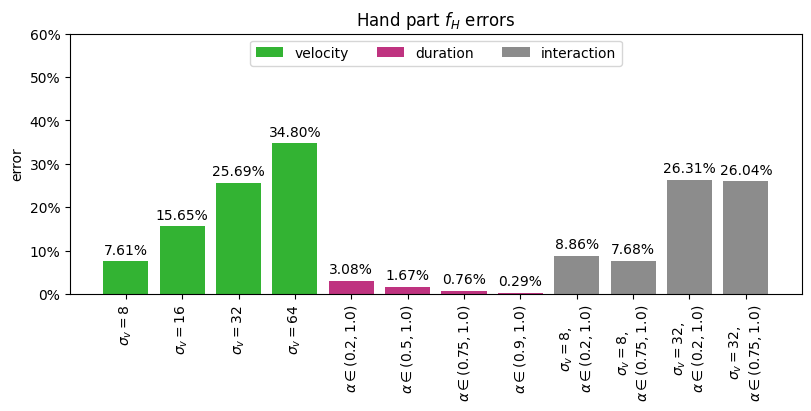
\includegraphics[width=0.7\textwidth]{images/ceteris_paribus_results_h.png}
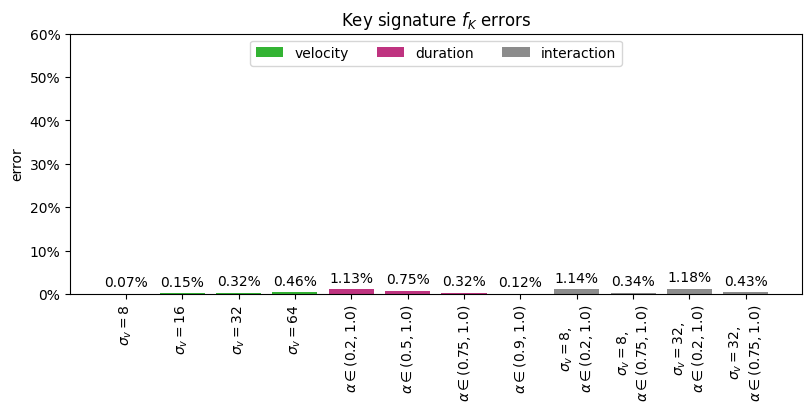
\includegraphics[width=0.7\textwidth]{images/ceteris_paribus_results_k.png}
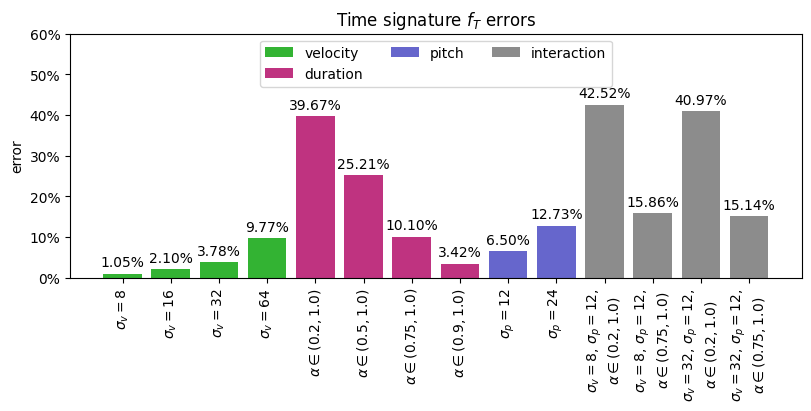
\includegraphics[width=0.7\textwidth]{images/ceteris_paribus_results_t.png}
\caption[Results of the \emph{ceteris paribus} experiment]{Results of the \emph{ceteris paribus} experiment for the hand part model $f_H$, the key signature model $f_K$ and the time signature model $f_T$. The hand part model is robust to note duration changes while it is susceptible to velocity manipulation. On the other hand, the time signature model is sensitive to note duration changes, which is expected to some extent, and relatively robust to other transformations. The key signature model is robust to all perturbations.}
\label{ceteris_paribus}
\end{figure}

Figure \ref{hand_part_misalignment} shows the result of hand part assignment for velocity perturbation.

\begin{figure}[!ht]
\centering
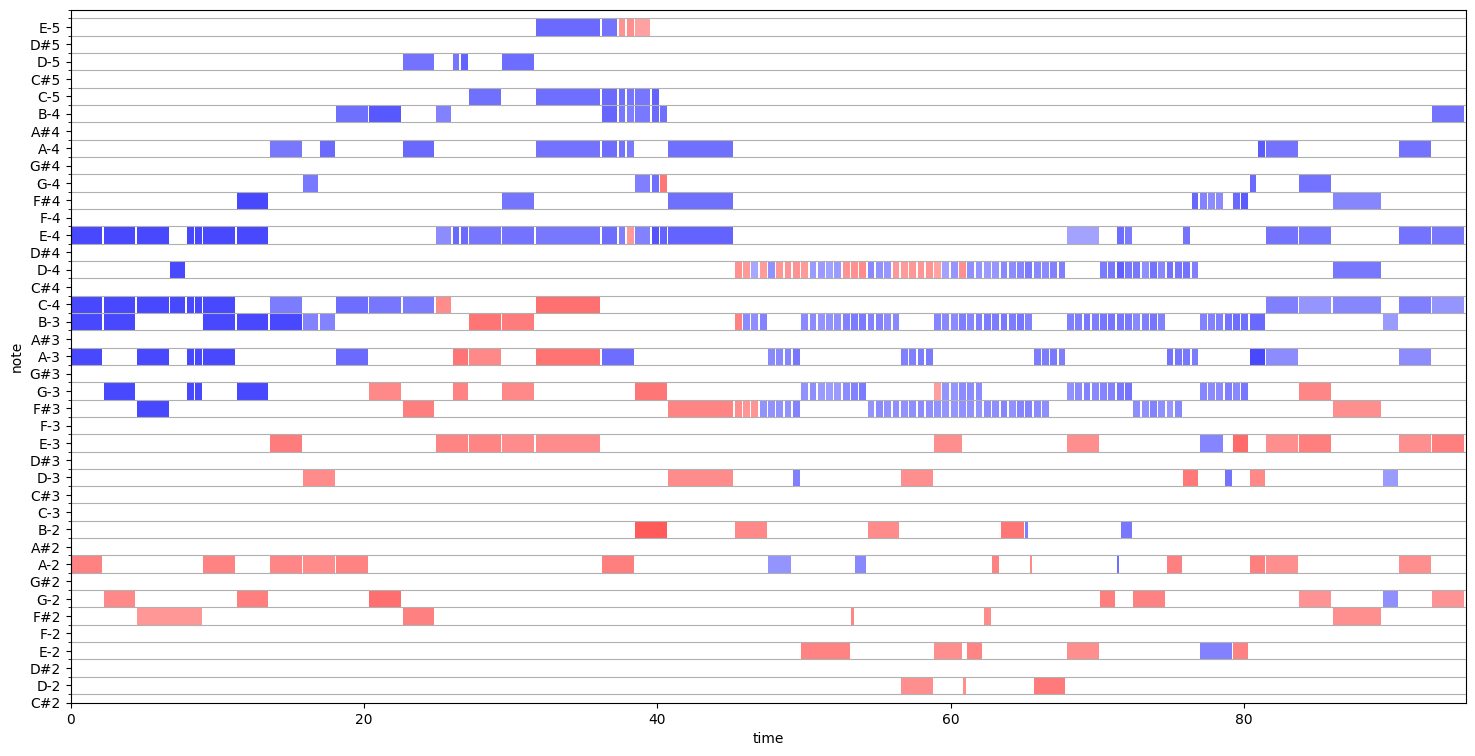
\includegraphics[width=0.95\textwidth]{images/hand_part1.png}
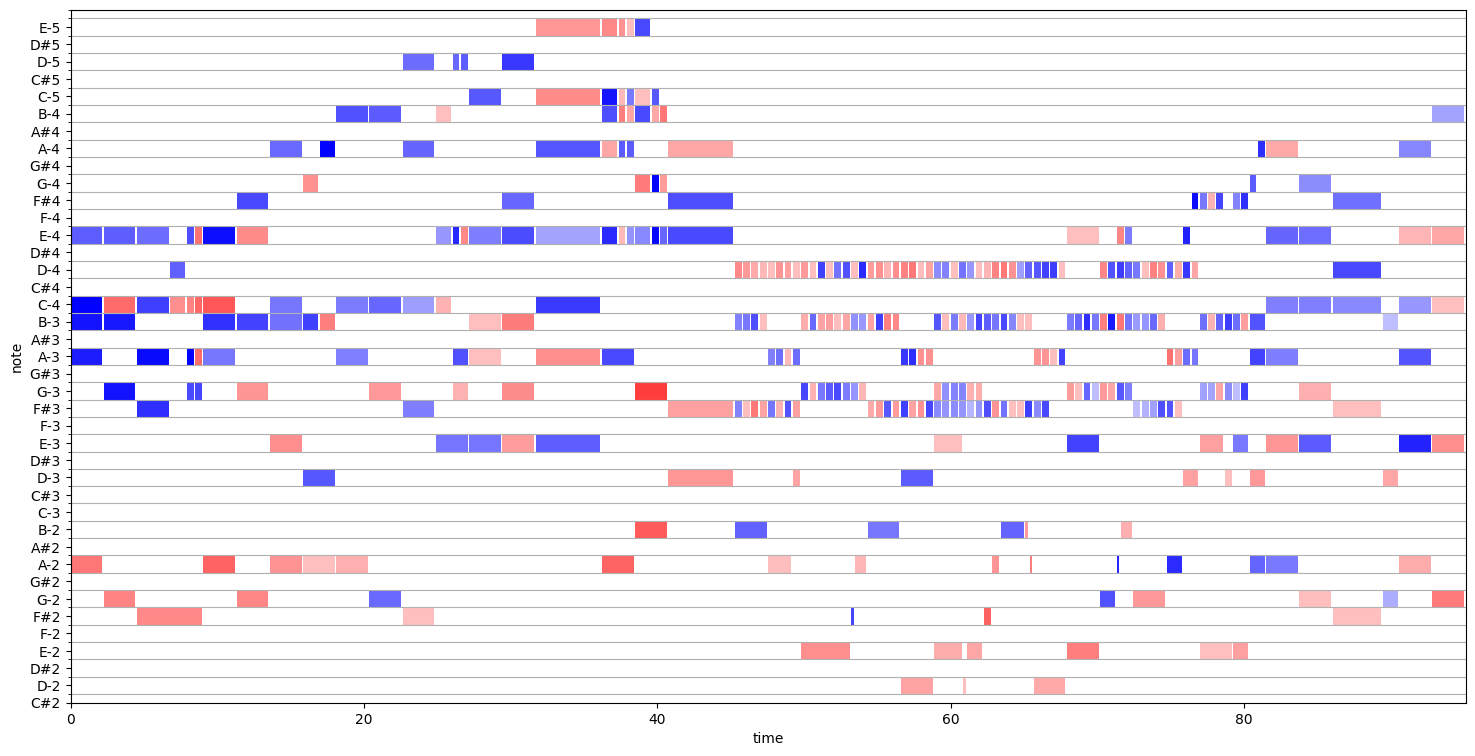
\includegraphics[width=0.95\textwidth]{images/hand_part2.png}
\caption[The piano roll for the hand part model output]{The piano roll for the hand part model output. Each note is represented as a (blue or red) block, indicating a pitch (note), duration and velocity. The first graph represents an original sequence while the second has perturbed velocity. Left-hand notes are marked as red. We can see that there are much many misalignment in the hand assignment in the second output. As a rule of thumb, the left hand notes (red) should be at the bottom while the right hand ones (blue) should be at the top.}\end{figure}

\section{Local Feature Importance}

[XAI]

To understand better the models' behavior, we tried to measure local influences of each feature onto models' decisions. In particularly, we posed several questions:

\begin{itemize}
	\item Is there any way to check which note features influenced models' decisions?
	\item Can we pinpoint notes that contribute the most to a model assignment, for example key signature attribution?
	\item Can we measure the strength and direction of a particular note feature? In particular, can we assign if a note feature voted for or against right hand assignment?
\end{itemize}

This type of questions, along with previous analysis, may help understanding the decision process of the model, facilitate recognizing weak spots of AMT systems and its limitations, and, finally, guide towards developing better AMT system.

We encountered challenges with common explainable machine learning tools: 

\begin{itemize}
	\item The input data is a very high-dimensional space, computationally infeasible for certain methods (e.g. Shapley values).
	\item Pitch space is a discrete space that lacks a meaningful measure of distance.
	\item Input data is a tensor of variable length, not conforming to tabular or image-like formats supported by many tools. Some model components (e.g. GRU blocks, ELU activation function) are not supported by certain XAI libraries. \missing
\end{itemize} 

We developed a custom solution to overcome these obstacles. For velocity, we applied a LIME-like approach due to the absence of metric structure in the pitch space. We generated a locally modified version of the MIDI stream tensor for each note, randomizing the velocity for one note. We created $100$ samples for each note, calculating model predictions to compare with the original prediction. This approach aids in explaining the findings from the previous section (see Figure \ref{hand_part_misalignment} for an example).

However, the proposed approach ignores the feature interaction and silently assumes variable independence, both horizontally and vertically. This is a serious limitation of this approach. 

\begin{figure}[!ht]
\centering
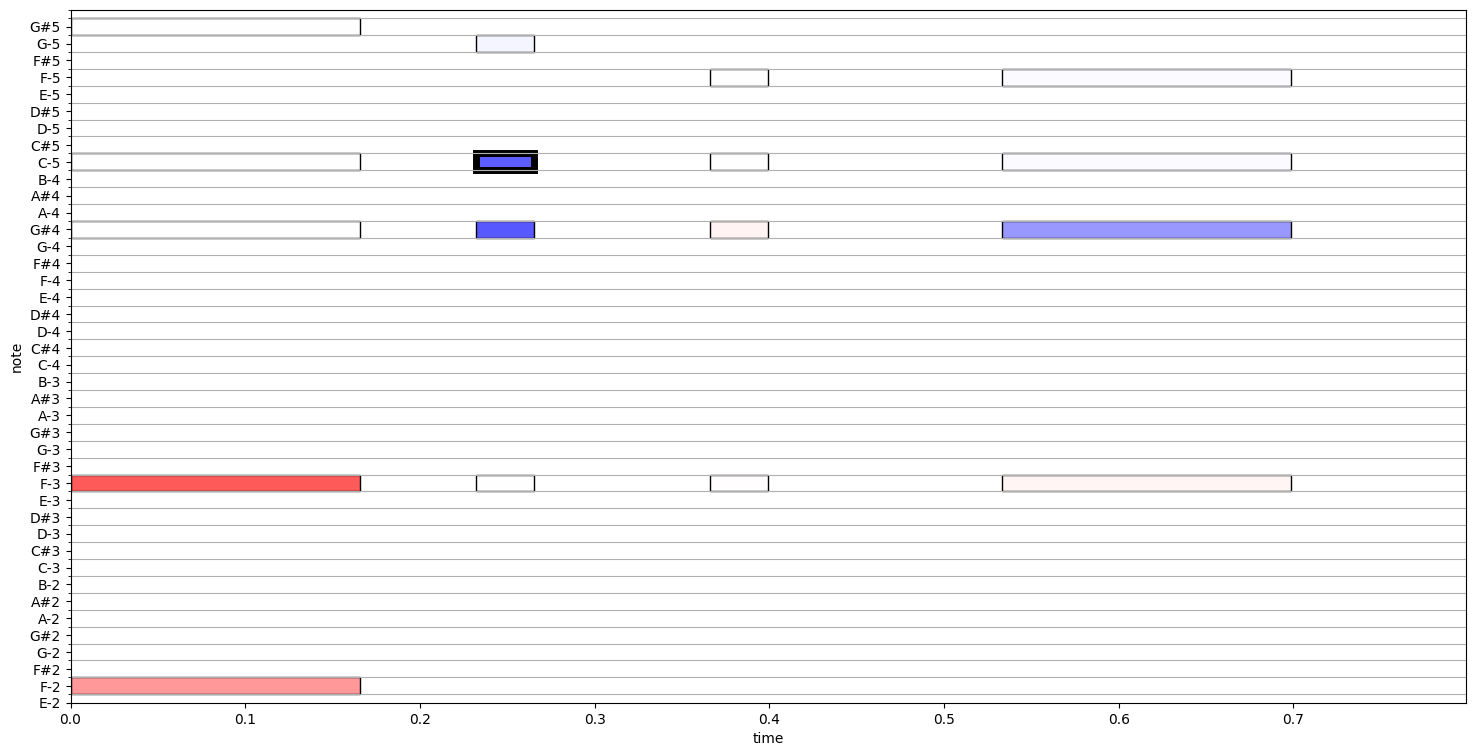
\includegraphics[width=0.95\textwidth]{images/lime_hand_part.png}
\caption[A graph showing how the velocity of a note influences hand part assignments of other notes]{A graph showing how the velocity of the second C5 note (with a thick outline) influences hand part assignments of other notes. It can be observed that the current velocity of this note makes the model think of the first F3 note as a left hand note. Reducing the note C5 velocity to a low value results in a misassigning F3 as the right hand note. This is, of course, a undesired behavior of the model.}
\label{hand_part_misalignment}\end{figure}

\subsection{Key Signature Assignment by Note Omission}

For the key signature model, as the pitch space is not a metric space, we applied a different strategy. The method is as follows: \begin{enumerate}
	\item Get the key signature prediction values (before the last activation function) for the entire sequence.
	\item Individually remove each note in a sequence and calculate the difference between the original prediction and the prediction made on a sequence without a single note.
	\item Compute a contribution score, represented by the mean of the differences for each note.
	\end{enumerate} This approach enables the measurement of each note's contribution to the attribution of a specific scale. Refer to Figure \ref{note_removing} for an illustrative example.

\begin{figure}[!ht]
\centering
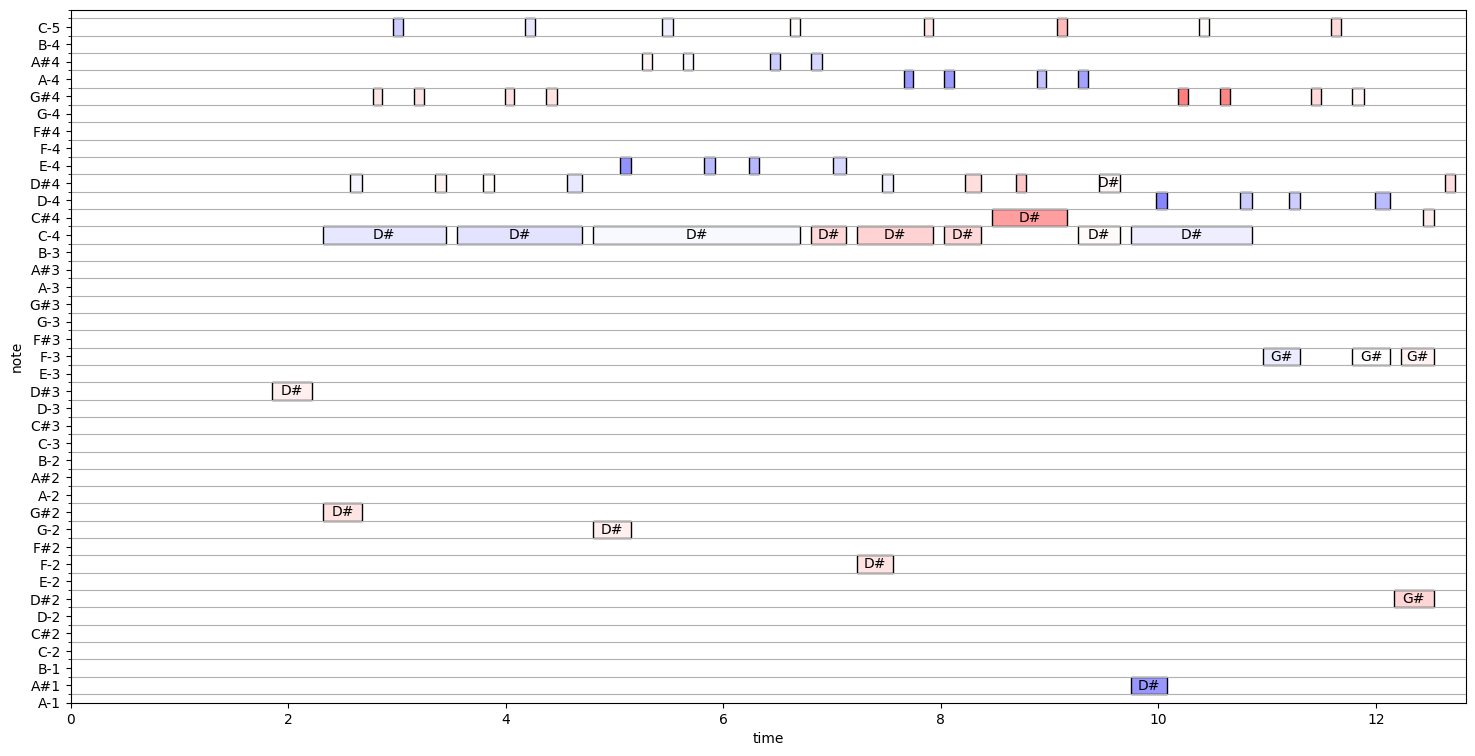
\includegraphics[width=0.95\textwidth]{images/note_removing.png}
\caption[A key signature alignment for D$\sharp$ scale]{A key signature alignment for D$\sharp$ scale. The names on the notes represent the model key signature attribution. There are two different scales assigned by the model: D$\sharp$ scale and G$\sharp$ scale. Notes: D, E and A are not in the scale and have a negative influence on the assignment.}
\label{note_removing}\end{figure}
	
\subsection{Ablation Studies} \label{ablation_studies}

In order to enforce Section \ref{robustness_analysis} assumptions, we trained a set of models that take only a limited number of features. More precisely: \begin{itemize}
	\item The \textbf{hand part} model has been trained only on note pitches and onsets.
	\item The \textbf{key signature} model has been trained only on note pitches and onsets.
	\item The \textbf{time signature} model has been trained only on note onsets.
\end{itemize}

As a result, all models became invulnerable to transformations described in the Section \ref{perturbations}. We are going to check check how such change affects the quality of models. 

Each model has been evaluated in two ways, using: \begin{itemize}
	\item model-specific $F_1$ metrics
	\item the MV2H metric
\end{itemize}

The MV2H metric has been evaluated on the set of all original models with one replaced. Only the test subset of the dataset has been used. For a fair comparison, both base and restricted models have been trained on the training set only.

For each ablation study, we picked the model that had the best $F_1$ score among all models trained in the span of 50 epochs.

\subsubsection{Beat Tracking} \label{beat_tracking}

The authors themselves provided ablation studies for the beat-tracking model. They analyzed how feature omission or data augmentation influences the beat-tracking model. The results of the analysis are provided in: Table \ref{beat_tracking_feature_omission} and Table \ref{beat_tracking_data_augmentation}.

\begin{table}[ht!]
\centering
\begin{tabular}{cccc}
    \textbf{Feature omitted} & Precision & Recall  & $F_1$ score   \\\hline
    Pitch                    & $0.904$   & $0.937$ & $0.906$       \\
    Onset                    & $0.846$   & $0.728$ & $0.764$       \\
    Duration                 & $0.895$   & $0.931$ & $0.901$       \\
    Velocity                 & $0.895$   & $0.939$ & $0.906$       \\
    Use all features         & $0.912$   & $0.943$ & ${\bf 0.913}$ \\
\end{tabular}

\caption[Feature omission study]{Feature omission study \cite{Liu2022}.}
\label{beat_tracking_feature_omission}
\end{table}

Not surprisingly, note onsets are the most important feature used by the beat-tracking model. While neglecting other features doesn't hardly impact the model, still feature omission results in a slight quality degradation.

Velocity may carry some information about beats as they tend to occur along with heavier notes \cite{Liu2022}. Harmonic structure inferred by pitch may also transfer such information, for example it is quite common to play chords at the beginning of a measure. On the other hand note durations may hint the metrical structure of a piece.

\begin{table}[ht!]
\centering
\begin{tabular}{cccc}
    \textbf{Augmentation method omitted} & Precision & Recall  & $F_1$ score      \\\hline
    Pitch shift                          & $0.920$   & $0.920$ & $0.906$          \\
    Tempo change                         & $0.918$   & $0.895$ & $0.897$          \\
    Note removal                         & $0.915$   & $0.909$ & $0.904$          \\
    Extra note insertion                 & $0.912$   & $0.943$ & $0.913$          \\
    Use all methods                      & $0.929$   & $0.937$ & $\mathbf{0.922}$ \\
    No data augmentation                 & $0.897$   & $0.952$ & $0.909$
\end{tabular}

\caption[Ablation study for data augmentation]{Ablation study for data augmentation \cite{Liu2022}.}
\label{beat_tracking_data_augmentation}
\end{table}

\subsubsection{Hand Part Model}

A variant of the hand part model that does not use neither durations nor velocities has been evaluated.

As the hand part affects only voice separation subscale of the MV2H metric, we omit remaining submetrics.

\begin{table}[ht!]
\centering
\begin{tabular}{ccc}
    \textbf{Metric}  & \textbf{Standard} & \textbf{Restricted} \\\hline
    Accuracy         & $0.956$           & $0.949$                \\
    Precision        & $0.851$           & $0.843$                \\
    Recall           & $0.848$           & $0.845$                \\
    $F_1$-score      & $0.842$           & $0.840$                \\
    Voice separation & $0.852$           & $0.818$                \\
\end{tabular}

\caption[The hand part model]{Comparison of the velocity-free hand part model and the original.}
\label{hand_part_ablation}
\end{table}

The results of both models are comparable (see the Figure \ref{hand_part_ablation}) in terms of $F_1$-score, although the voice separation MV2H submetric dropped. This suggests that the velocity may hint the hand assignment from time to time, but it is not (and it should not be) a direct indication of the

\subsection{Conclusion}

We were able to discover certain artifacts of the score generation models, especially when it comes to velocity contribution to hand part assignment. The time signature model is not fully robust to alterations that should not have affect the output.

Unfortunately, the proposed methods have drawbacks and are not fully justified. Current XAI methods do not work well with symbolic music data in general. Developing more tailored and adaptable XAI methods for musical applications could contribute to improved model interpretability. One of the challenge would be to find a reasonable (and interpretable) embedding of the pitch space that encodes musical features. 

